\chapter{IO-Ports}

\section{Einführung}

\paragraph*{Schaltung}
Das Schaltungungsbild zeigt, dass an den Bits Null bis Zwei des Ports vier 
jeweils eine LED so wie der zugehörige Vorwiederstand verschaltet ist. 
Die andere Seite der LEDs ist ist an die Stromquelle (mit vermutlich 3 V) 
angeschlossen. Das vierte Bit des Port vier ist an das Gate eines p-Kanal 
MOSFETs angeschlossen. Solange zwischen Gate und Source keine positive
Spannung anlegt leitet der MOSFET nicht. Die Source des MOSFET ist mit 
der Spannung verbunden. \\
Wird eine Null auf eine Portleitung geschrieben so liegt an ihr, wenn in
PXDIR das entsprechende Bit auf Ausgang steht (der Wert muss Eins sein), 
die Versorgungsspannung des Controllers an, anderenfalls Ground. \\
Wir auf die Bits der LEDs eine Null geschrieben so gibt es ein 
Spannungsgefälle in Leitrichtung der LED so dass ein Strom über die LED 
fließt und diese leuchtet. Anderes herum verhält es sich bei dem 
Lautsprecher; Damit dieser einen Ton ausgeben kann muss über den MOSFET
ein Strom fließen können, dies wird erreicht in dem auf das Gate Spannung 
gelegt wird durch schreiben einer Eins in die angeschlossene Protleitung.

\begin{figure}
\centering
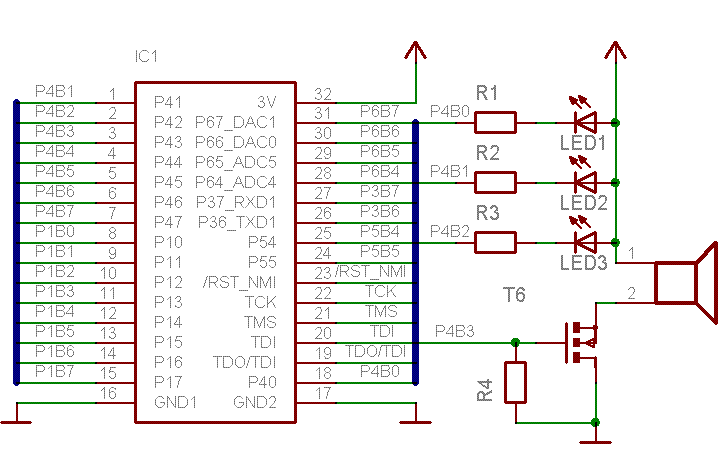
\includegraphics[width=0.5\textwidth]{img/mikrocontrollerUNDled.png}
\caption{\em \small Schaltplan mit LEDs und Lautsprecher}
\end{figure}

\section{Aufgabe 1}

\paragraph{} Die in der Aufgabenstellung gegebenen Befehle und 
ihre Wirkung sind in der folgenden Tabelle beschreiben:

\begin{longtable}{p{0.4\textwidth}p{0.5\textwidth}}

\textbf{Befehl} &
\textbf{Wirkung}
\endhead
\hline

\begin{lstlisting} 
#define LEDRT (0x01)
\end{lstlisting} &
Definition eines Präcompilermakros LEDRT.\\
\hline

\begin{lstlisting} 
P4DIR = 0x00; 
\end{lstlisting} &
Setzen der Ausgaberichtung des Portes 4 auf ausgehend.\\
\hline

\begin{lstlisting} 
a = 10;
\end{lstlisting} &
Die Variable a wird auf den dezimal Wert 10 gesetzt.\\
\hline

\begin{lstlisting} 
P4OUT = a;
\end{lstlisting} &
Schreibzugriff auf das Ausgaberegister des Ports 4. Es wird 00001010 
geschrieben, so dass das 2 und 4 Bit auf Spannung die anderen auf Ground
liegen.\\
\hline

\begin{lstlisting} 
P4OUT = 0x01; 
\end{lstlisting}  &
Erneuter Schreibzugriff auf Port 4 (genauer gesagt auf das 
Ausgaberegister).\\
\hline 

\begin{lstlisting} 
P4DIR = 0x0F;
\end{lstlisting}  &
In das Dir-Register des Portes 4 wird 11111111 geschrieben, so dass
alle Bits als Ausgabe benutzt wird. \\
\hline

\begin{lstlisting} 
a = P4IN & 0x0F;
\end{lstlisting}  &
Der Wert der am Port 4 wird mit 0x0F bitweise verundet und in a 
geschrieben. Das heißt dass die ersten 4 Bits in a genauso gesetzt 
sind wie in PIN, die anderen 4 Bits sind 0.\\
\hline 

\begin{lstlisting} 
P4OUT &= 0x08;
\end{lstlisting}  &
In das Ausgaberegister des Portes 4 wird das 4 Bit auf 1 gesetzt, falls
das Bit vorher schon 1 war, der Rest auf 0.\\
\hline 

\begin{lstlisting} 
P4OUT |= 0x01;
\end{lstlisting} &
Im Ausgaberegister des Portes 4 wird das erste Bit auf 1 gesetzt, der 
Rest beibehalten in dem das Register bitweise mit 00000001 verodert 
wird.\\
\hline

\begin{lstlisting} 
P4OUT |= LEDRT;
\end{lstlisting}  &
Unter Verwendung eines Präcompiler-Makros wird in P4OUT das erste Bit 
auf 1 gesetzt, und damit die angeschlossene LED ausschaltet.\\
\hline 

\begin{lstlisting} 
P4OUT &= ~LEDRT;
\end{lstlisting} &
Das erste Bit in P4OUT wird auf 0 gesetzt, und somit die angeschlossene
LED eingeschaltet.\\
\hline 

\begin{lstlisting} 
P4OUT ^= LEDRT;
\end{lstlisting}  &
Durch ein bitweises XOR wird das erste Bit in P4OUT getoggelt. Das 
heißt wenn das Bit vorher auf 0 war ist es nun 1 und umgekehrt. \\
\hline 

\end{longtable}


\lstinputlisting{src/aufgabe1.c}
\section{Aufgabe 2}
\lstinputlisting[caption=aufgabe2.c]{src/aufgabe2.c}
\section{Aufgabe 3}
\lstinputlisting[caption=aufgabe3.c]{src/aufgabe3.c}
\section{Aufgabe 4}
\lstinputlisting[caption=aufgabe4.c]{src/aufgabe4.c}
